% Figure from MATH 591 notes, section 39. Compile with the notes preamble.
\begin{tikzpicture}[scale=1.3]
\draw[->, gray!70!black] (-2.4,0) -- (2.4,0) node[right, font=\scriptsize, text=black] {$x$};
\draw[->, gray!70!black] (0,-0.3) -- (0,2.9) node[above, font=\scriptsize, text=black] {$y$};
\draw[blue, thick, domain=-1.6:1.6, samples=100, variable=\t] plot ({\t}, {(\t)*(\t)});
\draw[red, thick, domain=-0.82:0.82, samples=200, variable=\t] plot ({-4*(\t)*(\t)*(\t)}, {3*(\t)*(\t) + 0.5});
\fill (0,0.5) circle (1.5pt);
\node[font=\scriptsize, anchor=west] at (0.1,0.58) {$(0, \tfrac12)$};
\draw[blue, thick] (-2.2,-0.7) -- (-1.8,-0.7) node[right, font=\scriptsize, text=black] {parabola $y = x^2$};
\draw[red, thick] (0.3,-0.7) -- (0.7,-0.7) node[right, font=\scriptsize, text=black] {focal points $\mathbf{r}(a)$};
\end{tikzpicture}
